\documentclass{standalone}
\usepackage{tikz}
\begin{document}
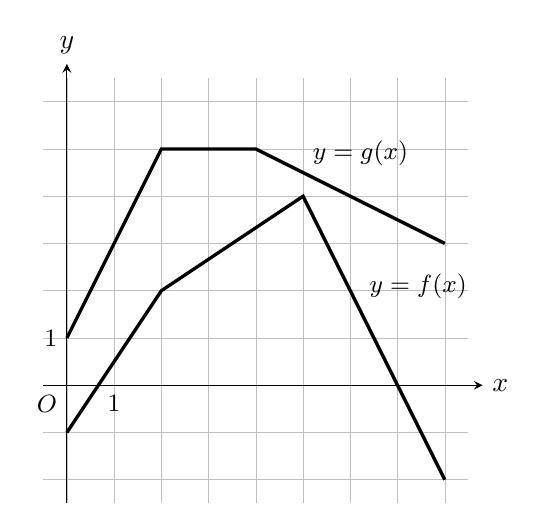
\begin{tikzpicture}[>=stealth, scale=0.6]
  % Gridlines
  \draw[help lines, gray!50] (-0.5,-2.5) grid (8.5,6.5);

  % Axes
  \draw[->] (-0.5,0) -- (8.8,0) node[right] {$x$};
  \draw[->] (0,-2.5) -- (0,6.8) node[above] {$y$};

  % g(x): (0,1) -> (2,5) -> (4,5) -> (8,3)
  \draw[very thick] (0,1) -- (2,5) -- (4,5) -- (8,3);
  % f(x): (0,-1) -> (2,2) -> (5,4) -> (8,-2)
  \draw[very thick] (0,-1) -- (2,2) -- (5,4) -- (8,-2);

  % Function labels
  \node[right,font=\small] at (5,4.9) {$y = g(x)$};
  \node[right,font=\small] at (6.2,2.1) {$y = f(x)$};

  % Axis labels
  \node[below left,font=\small] at (0,0) {$O$};
  \node[below,font=\small] at (1,0) {$1$};
  \node[left,font=\small]  at (0,1) {$1$};
\end{tikzpicture}
\end{document}
